\documentclass{article}

\usepackage{arxiv}
\usepackage{amsmath, amssymb}
\usepackage{graphicx}
\usepackage{hyperref}
\usepackage{algorithm}
\usepackage{algorithmic}
\usepackage{tikz}

\title{Dual Embedding Cross-Check (DEC): 
A Lightweight Method for Detecting LLM Semantic Drift and Hallucination}

\author{
  Raghvendran Kumar / Raghav Kumar \\
  Independent Explorer \\
  India \\
  \texttt{raghavk.azp@gmail.com}
}

\begin{document}
\maketitle

\begin{abstract}
Large language models (LLMs) possess impressive generative and reasoning capabilities 
but remain vulnerable to hallucination, semantic drift, and overconfident errors. 
Mitigation strategies such as larger model sizes, reinforcement learning, and retrieval augmentation 
increase computational cost, reduce interpretability, or require retraining.

We propose \textbf{Dual Embedding Cross-Check (DEC)}: a simple, low-cost method 
that compares the dynamic output embeddings of a transformer model with a stable, 
independent semantic space (e.g., Word2Vec, GloVe, FastText). 
Divergence between these two semantic trajectories provides an interpretable signal 
for detecting hallucination or drift.

DEC requires no model modification, no retraining, no GPU inference overhead, 
and minimal computation. It can act as an external semantic stabilizer, 
with the potential to make a 20B parameter model behave as reliably as a 70B model—
and give GPUs and RAM back to gamers.
\end{abstract}

\keywords{LLM, hallucination detection, vector semantics, embeddings, semantic drift, model reliability}

\section{Introduction}

Large language models have transformed natural language processing, enabling 
remarkably fluent generation and robust reasoning. Yet they remain fundamentally 
probabilistic systems; as a result, they can produce incorrect, fabricated, or 
internally inconsistent outputs. 

Recent research on hallucination has focused on:
\begin{itemize}
    \item scaling (larger models to reduce uncertainty),
    \item reinforcement learning from human or AI feedback,
    \item retrieval augmentation,
    \item ensembles and self-consistency mechanisms.
\end{itemize}

While these approaches improve reliability, they come at a cost:
computational expense, reduced transparency, and engineering complexity.

This paper introduces a simpler idea: 
\textbf{evaluate the model's semantic path using a second, stable embedding reference}.  
If the two semantic trajectories diverge, the model may be drifting into hallucination.

\section{Method: Dual Embedding Cross-Check (DEC)}

Transformers operate in a contextualized, high-dimensional vector space. 
The embedding of a token varies depending on surrounding context, internal attention distributions, 
model depth, and reasoning steps. This flexibility is powerful but introduces instability.

Static word-embedding models (Word2Vec, GloVe, FastText), in contrast, 
encode semantic relations that are fixed and stable across contexts.

DEC compares:
\begin{itemize}
    \item \textbf{Path A:} Transformer dynamic embeddings
    \item \textbf{Path B:} Static word-vector trajectory
\end{itemize}

If the transformer moves in a direction that meaningfully diverges from 
word-embedding semantic expectations, this may indicate hallucination or drift.

\subsection{Formal Definition}

Let $T = \{t_1, t_2, ..., t_n\}$ be tokens produced by an LLM.

Let $E_{LLM}(t_i)$ be the contextual embedding of $t_i$ from the transformer.

Let $E_{static}(t_i)$ be the nearest corresponding word-vector embedding in a static model.

We define two trajectories:

\[
P_{LLM} = (E_{LLM}(t_1), ..., E_{LLM}(t_n))
\]

\[
P_{static} = (E_{static}(t_1), ..., E_{static}(t_n))
\]

The DEC drift score is:

\[
D = 1 - \cos(P_{LLM}, P_{static})
\]

A threshold $\theta$ determines whether the drift is significant.

\section{Algorithm}

\begin{algorithm}[h]
\caption{Dual Embedding Cross-Check (DEC)}
\begin{algorithmic}[1]
\STATE \textbf{Input:} LLM embeddings $E_{LLM}$, static vectors $E_{static}$, threshold $\theta$
\FOR{each token embedding $v$ in $E_{LLM}$}
    \STATE Find nearest static embedding $u = \arg\max \cos(v, E_{static})$
    \STATE Append $u$ to the static trajectory
\ENDFOR
\STATE Compute drift score $D = 1 - \cos(P_{LLM}, P_{static})$
\IF{$D > \theta$}
    \RETURN ``Potential Hallucination'', $D$
\ELSE
    \RETURN ``Stable'', $D$
\ENDIF
\end{algorithmic}
\end{algorithm}

\section{Architecture Diagram}

Below is a conceptual flow (TikZ diagram may be inserted in final version):

\begin{center}
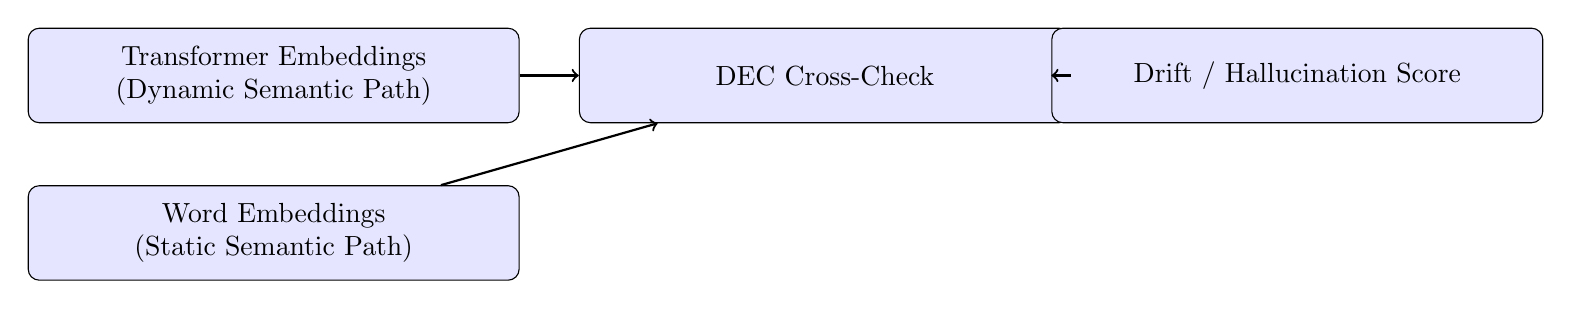
\begin{tikzpicture}[node distance=2cm, auto]
\tikzstyle{box} = [rectangle, rounded corners, draw=black, fill=blue!10, 
                   text width=6cm, text centered, minimum height=1.2cm]

\node[box] (transformer) {Transformer Embeddings (Dynamic Semantic Path)};
\node[box, below of=transformer] (static) {Word Embeddings (Static Semantic Path)};
\node[box, right of=transformer, xshift=5cm] (dec) {DEC Cross-Check};
\node[box, right of=dec, xshift=4cm] (output) {Drift / Hallucination Score};

\draw[->, thick] (transformer) -- (dec);
\draw[->, thick] (static) -- (dec);
\draw[->, thick] (dec) -- (output);
\end{tikzpicture}
\end{center}

\section{Applications}

\begin{itemize}
    \item Hallucination detection in reasoning chains
    \item Semantic drift detection over long contexts
    \item Safety and alignment monitoring
    \item Stabilizing mid-sized models (20B behaving like 70B)
\end{itemize}

\section{Limitations}

\begin{itemize}
    \item Word embeddings are coarse and not perfect semantic mirrors
    \item DEC is not a truth oracle
    \item May require task-specific threshold tuning
    \item Does not eliminate hallucinations; acts as an auxiliary signal
\end{itemize}

\section{Conclusion}

DEC is a simple, interpretable, compute-efficient method for monitoring 
semantic drift in large language models.  
By comparing transformer embeddings to an independent, stable vector space,  
DEC provides a lightweight signal that can flag potential hallucinations 
without modifying or retraining the underlying model.

\section*{References}

\begin{itemize}
    \item Mikolov et al., ``Efficient Estimation of Word Representations in Vector Space''
    \item Pennington et al., ``GloVe: Global Vectors for Word Representation''
    \item Vaswani et al., ``Attention is All You Need''
    \item Additional citations to be added in future versions
\end{itemize}

\end{document}
